\documentclass[a4paper,12pt]{article}
\usepackage[utf8]{inputenc}
\usepackage[T1]{fontenc}
\usepackage[french]{babel}
\usepackage{amsmath, amssymb}
\usepackage{graphicx}
\usepackage{hyperref}
\usepackage{float}
\usepackage{geometry}
\usepackage{fancyhdr}
\usepackage{caption}
\usepackage{graphicx}  % For images
\usepackage{hyperref}  % For hyperlinks
\usepackage{tikz}
\usepackage{capt-of}
\usepackage{listings}
\usepackage{xcolor}
\usepackage[utf8]{inputenc}  % Gestion UTF-8 (sous pdflatex)
\usepackage[T1]{fontenc}     % Encodage des fontes
\usepackage{amsmath}
\usepackage{array}        % pour les colonnes personnalisées (m{...}, >{...})
\usepackage[table]{xcolor} % pour la couleur des lignes
\usepackage{float}        % pour le [H] qui fige l’emplacement du tableau
\usepackage{ragged2e} 
\usepackage{tcolorbox}    % pour les encadrés
\usepackage{enumitem}     % pour personnaliser les listes



\geometry{margin=2.5cm}
\pagestyle{fancy}
\fancyhf{}
\rhead{Manuel Utilisateur - CubeSat}
\lhead{Détermination d’attitude}
\rfoot{\thepage}

% Couleurs pour le code
\definecolor{codegray}{rgb}{0.95,0.95,0.95}
\lstset{
    backgroundcolor=\color{codegray},
    basicstyle=\ttfamily\footnotesize,
    frame=single,
    breaklines=true,
    language=C
}

\begin{document}

% Page de garde
\begin{titlepage}
    \vspace*{\fill}  % Push content to the middle vertically
    \centering

    \begin{minipage}{0.45\textwidth}
        \centering
        
\includegraphics[width=0.6\textwidth]{fig/SU.jpg}
    \end{minipage}%
    \hfill
    \begin{minipage}{0.45\textwidth}
        \centering
        
\includegraphics[width=0.8\textwidth]{fig/Academie_Spatiale.png}
    \end{minipage}

    \vspace{5cm}

    {\bfseries\Huge Système de Détermination d’Attitude pour CubeSat\par}
\vspace{1cm}
    {\bfseries\Huge Manuel Utilisateur\par}
        \vspace{3cm}
    \textsc{\LARGE Sorbonne Université}\\[1cm]
    \textsc{\Large Académie Spatiale d'ile de France }\\[1cm]
    \textsc{\Large France 2030 }\\[1cm]
    \vspace{3cm}
    \textbf{Date: \today}

    \vspace*{\fill}  % Push bottom content to the bottom so that center aligns
\end{titlepage}
 \vspace*{\fill}
\begin{abstract}

Ce projet s’inscrit dans le contexte de l’Académie spatiale d’Île-de-France, projet financé par France 2030 visant à rattraper le retard de la France sur l’industrie.  L’Académie Spatiale d’Île-de-France a pour objectif de faire découvrir le spatial à la jeunesse française et à la communauté étudiante et de former les étudiants aux défis présents et futurs de l’industrie aérospatiale française.

 \vspace*{\fill}
\end{abstract}

\newpage
% Table of Contents
\tableofcontents
\newpage
\newpage

\section{Introduction}
Ce manuel presente \textbf{un système de determination d'attitude low-cost}, developpé pour un CubeSat \footnote{Un CubeSat dans sa forme basique, appelée 1U, c'est un cube de 10 × 10 × 10 centimètres de côté et dont la masse ne doit pas excéder deux kilogrammes.} \cite{noauthor_cubesat_2025}, ce système repose sur l'utilisation des \textbf{panneaux solaires} et un \textbf{magnétomètre 3 axes} connectés a un microcontrolleur \textbf{ESP32} pour l'acquisition et le traitement des données. Ce manuel décrit le matériel requis, les étapes d'installation, les instructions d'utilisation et les procédures de dépannage.

\section{Vue d’ensemble du système}
\subsection{Objectif technique}
Le système permet d'éstimer en temps réel l’attitude d’un cubesat en rotation par acquisition de la lumière du soleil et du champ magnétique terrestre.

\subsection{Application}
Le système est conçu pour des mission à petit budget (ex: projets universitaires, missions academiques, laboratoires de recherche)

\subsection{Fonctionnalités principales}
\begin{itemize}
 \item Mesure du champ magnétique terrestre 3 axes (BMM150)
 \item Détection de l’orientation solaire via 6 panneaux
 \item Filtrage du bruit 
 \item Calcul du vecteur Soleil-Satellite
 \item Representation 3D du vecteur Soleil-Satellite et du vecteur Magnetique
\end{itemize}

\subsection{Spécifications techniques}
\begin{table}[H]
\centering
\renewcommand{\arraystretch}{1.3}
\begin{tabular}{|>{\raggedright\arraybackslash}m{4.5cm}|>{\raggedright\arraybackslash}m{8.5cm}|}
\hline
\rowcolor{blue!10}
Alimentation & 3.3Vdc \newline Référence 0Vdc \\

\rowcolor{blue!5}
Dimensions & 10 × 10 × 10 centimètres \\

\rowcolor{blue!10}
Microcontrôleur & ESP32 – WROOM – 32, fréquence jusqu’à 240 MHz  \\

\rowcolor{blue!5}
Taux d’échantillonnage & 77kHz \\

\rowcolor{blue!10}
Format de sortie & Vecteurs normalisés \newline Format CSV \\

\rowcolor{blue!5}
Interfaces de communication & I2C pour le magnétomètre \newline Entrées analogiques pour les panneaux solaires \\
\hline
\end{tabular}
\caption{Spécifications techniques du système }
\label{tab:specs}
\end{table}


\subsection{Composants principaux}
\begin{table}[H]
\centering
\renewcommand{\arraystretch}{1.3}
\begin{tabular}{|>{\raggedright\arraybackslash}m{4.5cm}|>{\raggedright\arraybackslash}m{8.5cm}|}
\hline
\rowcolor{blue!30}
\textbf{Composant} & \textbf{Description} \\
\hline
\rowcolor{blue!10}
Microcontrôleur ESP32 & Alimentation : 3.3Vdc / 5Vdc (USB-C) / 5Vdc-12Vdc (pins) \newline Fréquence : 80-240MHz \newline Température de fonctionnement : -20°C à 85°C \newline Mémoire : 4Mbits Flash + 512Kbits SRAM \\

\rowcolor{blue!5}
BMM150 – Magnétomètre 3 axes & Communication I2C \newline Alimentation : 3.3V–5V \newline Température de fonctionnement : -40°C à 85°C \newline Plage de mesure : ±1300 µT \\

\rowcolor{blue!10}
Panneaux Solaires & Tension de charge maximale : 6,4V \newline Tension de circuit ouvert : 8,2V \newline Courant typique : 100 mA \newline Tension typique : 5,5V \newline Puissance : 0.5W \\
\hline
\end{tabular}
\caption{Détails des composants utilisés dans le système}
\label{tab:specs}
\end{table}


\section{Installation matérielle}
\subsection{Schema électrique}
\begin{figure}[H]  % Use [H] to place exactly here (requires the float package)
    \centering
    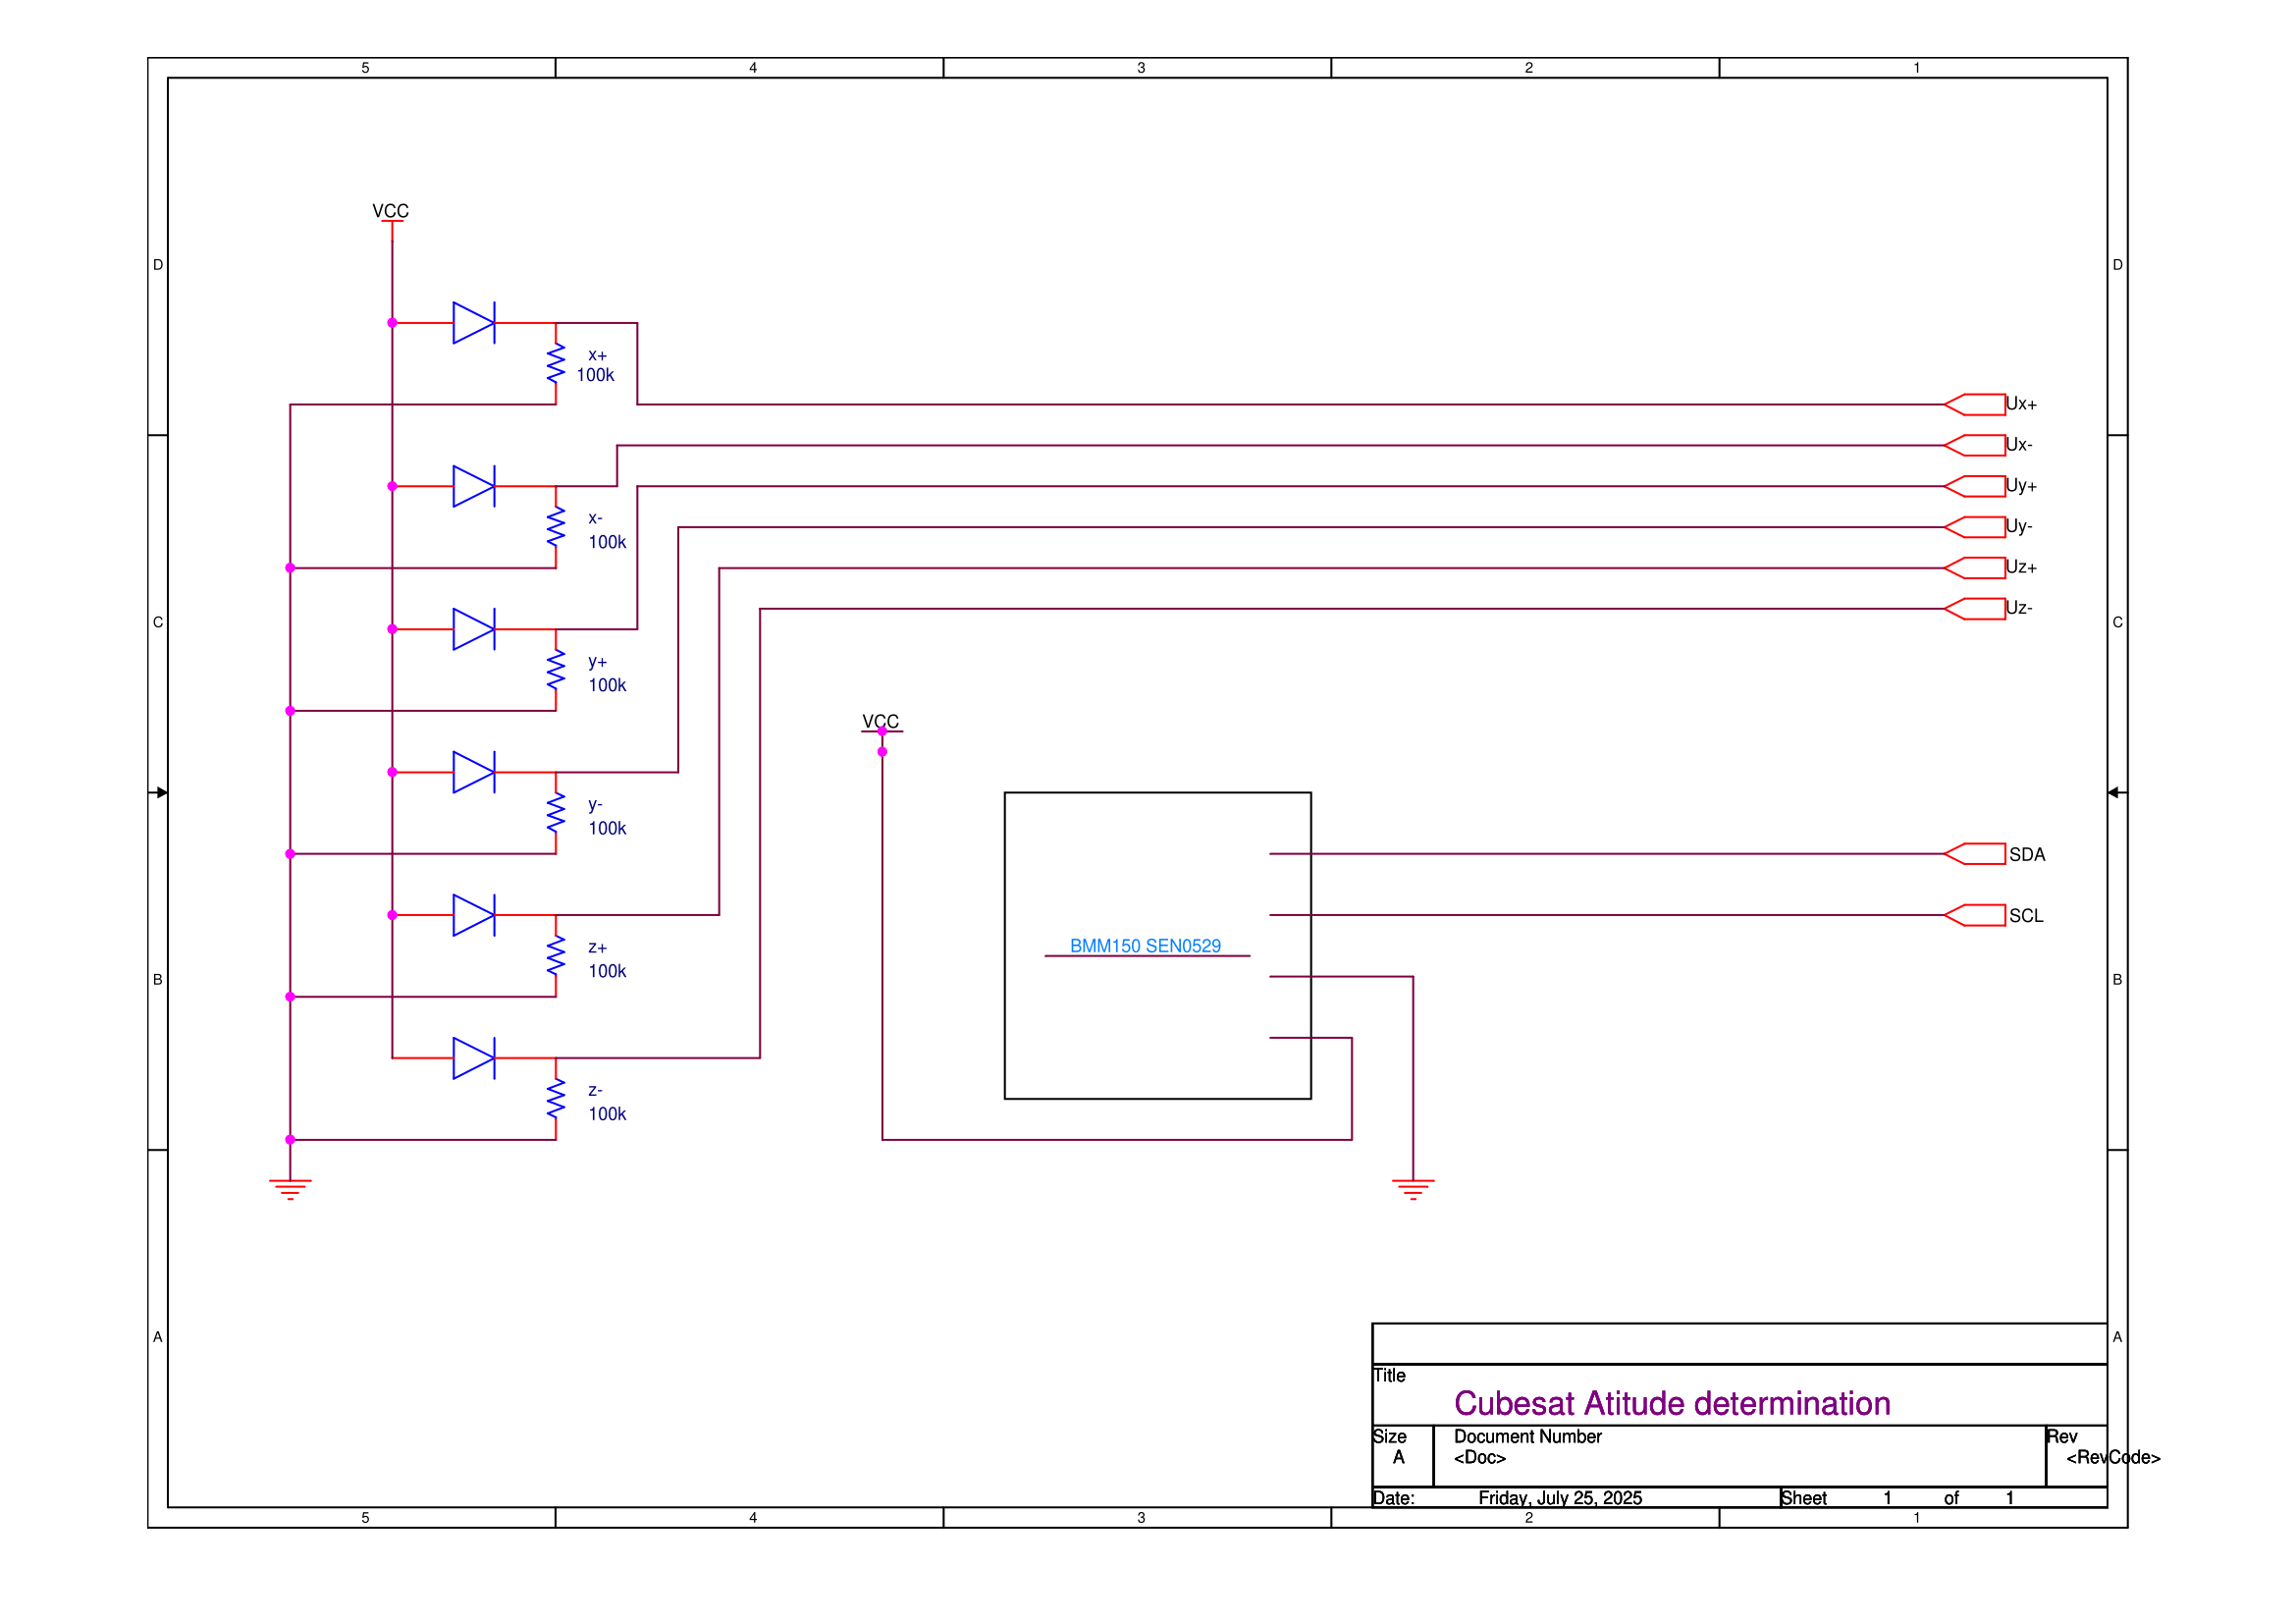
\includegraphics[width=0.9\textwidth]{fig/cubesatSchematic.png}
    \caption{Schema électrique}
    \label{fig:Schema électrique}
\end{figure}

\section{Mise en route logicielle}
\subsection{Prérequis}
\begin{itemize}
    \item IDE : \texttt{Espressif IDE} installé
    \item Drivers USB pour ESP32
    \item Dépendances (librairies I2C, capteur BMM150, etc.)
\end{itemize}

\subsection{Téléversement du code}
\begin{lstlisting}
// Dans ESP-IDF CMD
idf.py build
idf.py -p /dev/ttyUSB0 flash
idf.py monitor
\end{lstlisting}

\section{Utilisation du système}

\begin{enumerate}
    \item Brancher l’ESP32
    \item Ouvrir le moniteur série
    \item Observer les vecteurs affichés (Soleil, Champ magnétique)
\end{enumerate}

\subsection{Résultats Finale}

\begin{itemize}
    \item Affichage 3D du vecteur champ magnétique.
    \item Affichage 3D du vecteur Soleil-Satellite calculé à partir des panneaux solaires.
    \item Un Fichier CSV contenant l'evolution des deux vecteurs dans le temps.
\end{itemize}

\section{Dépannage}
\begin{itemize}
    \item \textbf{Aucune donnée du capteur} : vérifier l'adresse I2C et les connexions.
    \item \textbf{Luminosité nulle} : vérifier les résistances pull-down et l'exposition des panneaux.
    \item \textbf{ESP32 ne répond pas} : vérifier le câble USB et redémarrer la carte.
\end{itemize}

\newpage
\section{Précautions}

Afin de garantir le bon fonctionnement du système, il est important de respecter les consignes suivantes :\\[0.3cm]

\begin{enumerate}[label=\textbf{\arabic*.}, leftmargin=1.5cm]
    \item \textbf{Respecter la tension d’alimentation} \\
    Ne jamais alimenter la carte ESP32 ou les capteurs avec une tension supérieure à \textbf{3.3V} sur les broches logiques. \\
    Seule l’entrée USB (5V) est tolérée grâce au régulateur intégré. \\
    Une tension trop élevée appliquée directement sur les broches \texttt{3V3}, \texttt{GPIO} ou \texttt{I2C} peut \textbf{détruire le microcontrôleur}.\\[0.3cm]
    
    \item \textbf{Éviter les erreurs de câblage} \\
    Toujours vérifier les connexions avant de mettre sous tension. \\
    Ne jamais inverser les broches \texttt{GND} et \texttt{VCC} (erreur fréquente). \\
    Éviter les courts-circuits entre les broches (utiliser des breadboards ou connecteurs fiables).\\[0.3cm]
    
    \item \textbf{Éviter les pics de courant} \\
    Ne pas connecter ou déconnecter des composants pendant que le système est sous tension. \\
    Éviter les charges inductives sans protection (diode de roue libre, etc.).\\[0.3cm]
    
    \item \textbf{Manipuler les capteurs avec précaution} \\
    Ne pas exposer le magnétomètre à des champs magnétiques intenses artificiels. \\
    Protéger les capteurs contre les chocs et vibrations excessives. \\
    Éviter d'éblouir les photodiodes avec une lumière non naturelle.\\[0.3cm]
    
    \item \textbf{Programmer avec prudence} \\
    S'assurer que le code téléversé respecte la configuration des broches. \\
    Tester les modifications sur une maquette avant de les appliquer à l’ensemble du système.\\[0.3cm]
\end{enumerate}

\vspace{0.5cm}

\begin{tcolorbox}[colback=red!5!white, colframe=red!75!black, title=Important]
Une mauvaise manipulation ou une erreur de câblage peut entraîner des \textbf{dommages irréversibles} à la carte ESP32 ou aux capteurs. Prenez toujours le temps de \textbf{vérifier deux fois} avant de mettre sous tension.
\end{tcolorbox}


\section{Annexes}
\subsection{Extraits de code importants}
\begin{lstlisting}
// Fonction de lecture du capteur BMM150
bmm.read_mag_data();
\end{lstlisting}

\subsection{Ressources utiles}
\begin{itemize}
    \item \href{https://docs.espressif.com/projects/esp-idf/en/latest/}{Documentation officielle ESP-IDF}
    \item \href{https://wiki.dfrobot.com/SEN0529_BMM150_3-Axis_Magnetic_Field_Sensor_SKU_SEN0529}{Page produit BMM150}
\end{itemize}

\newpage

% References
\addcontentsline{toc}{section}{References}
\bibliographystyle{plain}
\bibliography{Determination_attitude}  % Create a references.bib file if needed

\end{document}
